\SourcePage{236}{239}
\section{Transition probability in the quasiclassical case}

Passage through a potential barrier is an example of a process that is wholly
impossible in classical mechanics. In the quasiclassical case the probability
of such processes is exponentially small. The corresponding exponential
factor can be found as follows.

When considering the transition of some system from one state to another, we
solve the corresponding classical equations of motion and find the transition
``trajectory,'' which is complex, however, in keeping with the impossibility
of the process in classical mechanics. In particular, the ``transition
point'' $q_0$, at which the formal change of the system from one state to the
other occurs, is generally complex; its position is fixed by the classical
conservation laws. We then calculate the action
$S_1(q_1,q_0)+S_2(q_0,q_2)$ for motion of the system in the first state from
some initial position $q_1$ to the ``transition point'' $q_0$, and subsequently
in the second state from $q_0$ to the final position $q_2$. The probability of
the process in question is then given by
\begin{equation}
 w\sim\exp\left\{-\frac2\hbar\operatorname{Im}
 [S_1(q_1,q_0)+S_2(q_0,q_2)]\right\}.
 \tag{52.1}
\end{equation}

If the position of the ``transition point'' is not unique, the one for which
the exponent in (52.1) has the smallest absolute value must be selected (while
this value must, of course, still be sufficiently large for formula (52.1) to
be applicable at all)\footnote{If the potential energy of the system itself
has singular points, these too must be included among the competing values of
$q_0$.}.

Formula (52.1) agrees with the rule obtained in the preceding section for
calculating quasiclassical matrix elements. It must be stressed, however, that
it would be incorrect to calculate the pre-exponential factor in the
probability of transitions of this kind from the square of the corresponding
matrix element.

The method of \emph{complex classical trajectories} based on (52.1) is quite
general and applies to transitions in systems with any number of degrees of
freedom (L.~D. Landau,

\SourcePage{237}{240}
1932). If the transition point is real but lies in a classically inaccessible
region, then, in the simplest case of one-dimensional motion, formula (52.1)
coincides with expression (50.5) for the probability of passage through a
potential barrier.

\textbf{Over-barrier reflection.} Let us apply (52.1) to the one-dimensional
problem of over-barrier reflection---the reflection of a particle whose energy
exceeds the height of the barrier. Here $q_0$ is to be understood as the
complex coordinate $x_0$ of the ``stopping point,'' at which the particle
reverses the direction of its motion, that is, a complex root of
$U(x)=E$. We shall show how in this case the reflection coefficient can also
be calculated more accurately, including the pre-exponential factor.

Once again (as in \S~50), we must establish the correspondence between the
wave functions far to the right of the barrier (the transmitted wave) and far
to its left (incident $+$ reflected waves). This is readily done by a method
similar to that already used in \S~47 and 50, treating $\psi$ as a function of
the complex variable $x$.

Write the transmitted wave as
\[
 \psi_+=\frac1{\sqrt p}\exp\left(\frac i\hbar\int_{x_1}^x p\,dx\right)
\]
(where $x_1$ is any point on the real axis), and follow its change during
continuation in the upper half-plane along a path $C$ which goes round the
turning point $x_0$ (at a sufficiently large distance), Fig.~19. The final
part of this path must lie entirely in a region sufficiently far to the left
that, along it, the error in the approximate (quasiclassical) wave function of
the incident wave is smaller than the small quantity $\psi_-$ being sought.
Going round $x_0$ changes the sign of the root $\sqrt{E-U(x)}$; consequently,
on returning to the real axis, $\psi_+$ becomes a wave $\psi_-$ propagating to
the left, that is, the reflected wave\footnote{Continuation along a path
passing below $x_0$ (for example, simply along the real axis itself) instead
turns $\psi_+$ into the incident wave.}. Since the amplitudes of the incident
and transmitted waves may be regarded as equal, the required reflection
coefficient $R$ is simply

\begin{figure}[ht]
\centering
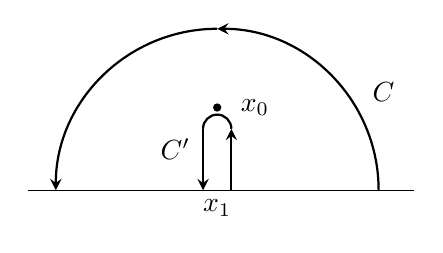
\begin{tikzpicture}[x=1cm,y=1cm,>=stealth]
 \draw (-2.4,0)--(2.5,0);
 \fill (0,1.05) circle (1.5pt) node[right=5pt] {$x_0$};
 \node[below] at (0,0) {$x_1$};
 \draw[thick,->] (2.05,0) arc[start angle=0,end angle=90,radius=2.05];
 \draw[thick,->] (0,2.05) arc[start angle=90,end angle=180,radius=2.05];
 \node[right] at (1.85,1.25) {$C$};
 \draw[thick,->] (0.18,0)--(0.18,.78);
 \draw[thick] (0.18,.78) arc[start angle=0,end angle=180,radius=.18];
 \draw[thick,->] (-.18,.78)--(-.18,0);
 \node[left] at (-.22,.52) {$C'$};
\end{tikzpicture}
\par\smallskip Fig. 19
\end{figure}

\SourcePage{238}{241}
the ratio of the squared moduli of $\psi_-$ and $\psi_+$:
\begin{equation}
 R=\left|\frac{\psi_-}{\psi_+}\right|^2
 =\exp\left(-\frac2\hbar\operatorname{Im}\int_Cp\,dx\right).
 \tag{52.2}
\end{equation}

Once this formula has been obtained, the integration path in the exponent may
be deformed arbitrarily. If it is changed into the path $C'$ shown in Fig.~19,
the integral reduces to twice the integral along the path from $x_1$ to $x_0$,
and we obtain
\begin{equation}
 R=e^{-4\sigma(x_1,x_0)/\hbar},\qquad
 \sigma(x_1,x_0)=\operatorname{Im}\int_{x_1}^{x_0}p(x)\,dx;
 \tag{52.3}
\end{equation}
since $p(x)$ is real over the entire real axis, the choice of $x_1$ is
immaterial\footnote{In some cases not only the amplitude relation but also the
phase relation between the incident and reflected waves is of interest. These
relations are characterized by the reflection amplitude, expressed in terms
of the coefficients $\alpha$ and $\beta$ introduced in \S~25. The reasoning
given above readily shows, in particular, that the reflection amplitude for a
wave incident from the left is
\[
 \left(-\frac{\beta^*}{\alpha^*}\right)
 =-i\exp\left[\frac{2i}{\hbar}\left(
 \int_{x_1}^{x_0}p\,dx+p_1x_1\right)\right],\qquad x_1\to-\infty.
\]
(The factor $(-i)$ is associated with the change in phase of the
pre-exponential factor on going round the branch point; compare \S~47.)}.
Notice that the pre-exponential factor in (52.3) is equal to unity
(V.~L. Pokrovsky, S.~K. Savvinykh, F.~R. Ulinich, 1958)\footnote{The
derivation of this result presented here is due to L.~D. Landau (1961).}.

As already stated, among all possible values of $x_0$ one must choose that for
which the exponent in (52.3) has the smallest absolute value, while this value
must still be sufficiently large compared with unity. (Only points $x_0$ for
which $\sigma>0$, that is, points lying in the upper half-plane, are of course
to be considered.) It is also assumed that if the potential energy $U(x)$
itself has singular points in the upper half-plane, the integrals
$\sigma(x_1,x_0)$ for them are large\footnote{The contour $C$ in Fig.~19 must
pass below the singular points of $U(x)$.}. Otherwise such a point itself
determines the exponent, but the pre-exponential coefficient is then no longer
the one in (52.3). The latter condition necessarily fails as the energy $E$ is
increased if $U(x)$ becomes infinite somewhere

\SourcePage{239}{242}
in the upper half-plane: a stage is reached at which the point $x_0$, where
$U=E$, approaches the point $x_\infty$, where $U=\infty$, so closely that the
two give comparable contributions to the reflection coefficient
($\sigma(x_\infty,x_0)\sim1$), and formula (52.3) ceases to apply. In the
limiting case, when $E$ is so large that this integral is small compared with
unity, perturbation theory becomes applicable (see Problem~2)\footnote{The
intermediate case was considered by V.~L. Pokrovsky and I.~M. Khalatnikov
(ZhETF, 1961, vol.~40, p.~1713).}.
